\documentclass[12pt,a4paper]{article}
\usepackage[margin=1in]{geometry}
\usepackage{amsmath,amssymb,bm}
\usepackage{graphicx}
\usepackage{booktabs}
\usepackage{float}
\usepackage{algorithm}
\usepackage{algpseudocode}
\usepackage{hyperref}
\usepackage{siunitx}
\usepackage{tikz}
\usetikzlibrary{arrows.meta,positioning,shapes.geometric}

\usepackage[edges]{forest}
\usetikzlibrary{arrows.meta,shapes.geometric}
\tikzset{
  decision/.style={draw,diamond,aspect=2,inner sep=1pt,align=center},
  block/.style={draw,rounded corners,inner sep=3pt,align=center,text width=26mm}
}


\title{Methodology: Enhanced Genetic Algorithm with Adaptive Controllers (GAWorker)}
\date{}

\begin{document}
\maketitle

\section{Optimization Problem}
Let $\bm{x} = (x_1,\ldots,x_d)^\top$ denote the decision vector of DVA parameters. For each gene $i$ we have lower/upper bounds $\ell_i, u_i$ and an optional fixed value $c_i$. The feasible set is
\[ x_i = c_i \;\; (i \in \mathcal{F}) , \quad x_i \in [\ell_i,u_i] \;\; (i \notin \mathcal{F}) , \]
where $\mathcal{F}$ is the index set of fixed parameters.

The FRF model maps parameters to a scalar performance indicator (``singular response'') $s(\bm{x};\Theta)$ over a frequency grid $\Omega=[\omega_{\min},\omega_{\max}]$ with $N_\omega$ points, using main system parameters $\Theta$. In addition, target criteria across masses yield percentage differences $\Delta_{m,k}(\bm{x})$ (absolute percent errors) for mass index $m\in\{1,\ldots,5\}$ and criterion $k$.

The scalar fitness minimized by GAWorker is
\begin{equation}
\label{eq:fitness}
f(\bm{x}) = \underbrace{\left| s(\bm{x};\Theta) - 1\right|}_{\text{primary objective}} + \underbrace{\alpha \sum_{i=1}^{d} |x_i|}_{\text{sparsity penalty}} + \underbrace{\frac{1}{S} \sum_{m} \sum_{k} |\Delta_{m,k}(\bm{x})|}_{\text{percentage error term}},
\end{equation}
where $\alpha\ge 0$ is the sparsity weight (named \texttt{alpha} in code) and $S>0$ is a scaling factor (\texttt{percentage\_error\_scale}). The algorithm terminates early when $\min f \le \varepsilon$ (tolerance \texttt{ga\_tol}) or when the generation budget is reached.

\paragraph{Diversity and statistics.} Per generation, GAWorker computes population statistics:
\begin{align}
\mu &= \frac{1}{|\mathcal{P}|} \sum_{i\in \mathcal{P}} f_i, \label{eq:mean_fitness} \\
\sigma &= \sqrt{\frac{1}{|\mathcal{P}|} \sum_{i\in \mathcal{P}} f_i^2 - \mu^2}, \label{eq:std_fitness} \\
cv &= \frac{\sigma}{|\mu|+\varepsilon}, \label{eq:coefficient_variation}
\end{align}
and a gene-level diversity metric:
\begin{equation}
D = \frac{1}{d} \sum_{j=1}^{d} \min\!\left(1,\max\!\left(0, \frac{\sigma_j}{u_j-\ell_j}\right)\right), \label{eq:gene_diversity}
\end{equation}
where $\sigma_j$ is the per-gene standard deviation across the population.

\section{Initialization (Seeding)}
GAWorker supports multiple seeding strategies with fixed-parameter handling. Each method is implemented with careful consideration of fixed parameters and parameter bounds.

\subsection{Random Uniform Seeding}
\textbf{Mathematical Formulation:}
For each parameter $i = 1, \dots, d$:
\begin{equation}
x_i = \begin{cases}
c_i & \text{if } i \in \mathcal{F} \text{ (fixed parameter)} \\
\mathcal{U}(\ell_i, u_i) & \text{if } i \notin \mathcal{F} \text{ (variable parameter)}
\end{cases} \label{eq:random_seeding}
\end{equation}
where $\mathcal{U}(a,b)$ denotes the continuous uniform distribution on $[a,b)$.

\textbf{Implementation Details:}
\begin{enumerate}
\item Uses Python's \texttt{random.uniform()} for sampling each parameter value
\item Applied independently to each parameter without considering relationships between them
\item Fixed parameters (those marked as non-optimizable) are enforced exactly at their specified values
\item No correlation between parameters - each parameter is sampled completely independently
\item Computational complexity: $O(d)$ per individual, where $d$ is the number of parameters
\end{enumerate}

\textbf{Parameter Explanations:}
\begin{itemize}
\item $\bm{x} = (x_1, \dots, x_d)^\top$: The decision vector containing all $d$ parameters to be optimized
\item $\ell_i, u_i$: The lower and upper bounds for parameter $i$, defining the allowable range
\item $\mathcal{F}$: The set of indices for parameters that are fixed and cannot be changed during optimization
\item $c_i$: The fixed value for parameter $i$ when $i \in \mathcal{F}$
\item $d$: The total number of parameters in the optimization problem
\end{itemize}

\subsection{Sobol Quasi-Monte Carlo Seeding}
\textbf{Mathematical Formulation:}
\begin{enumerate}
\item Generate $n$ points from Sobol sequence in $[0,1]^d$: $\bm{z}^{(1)}, \dots, \bm{z}^{(n)}$
\item Scale to parameter bounds:
\begin{equation}
x_i^{(j)} = \ell_i + z_i^{(j)} \cdot (u_i - \ell_i) \quad \forall i,j \label{eq:sobol_scaling}
\end{equation}
\item Apply fixed parameters:
\begin{equation}
x_i^{(j)} = c_i \quad \forall i \in \mathcal{F}, \forall j \label{eq:sobol_fixed}
\end{equation}
\end{enumerate}

\textbf{Implementation Details:}
\begin{enumerate}
\item Uses \texttt{scipy.stats.qmc.Sobol} with scramble=True for improved uniformity and reduced correlation
\item Supports high dimensionality up to 40+ parameters efficiently
\item Reproducible results when a seed parameter is provided
\item Low-discrepancy property ensures even coverage of the parameter space
\item Computational complexity: $O(n \cdot d)$, linear in both population size and dimension
\end{enumerate}

\textbf{Parameter Explanations:}
\begin{itemize}
\item $\bm{z}^{(j)} = (z_1^{(j)}, \dots, z_d^{(j)})^\top$: A point in the d-dimensional unit hypercube $[0,1]^d$
\item $n$: The number of individuals (solutions) to generate for the initial population
\item $\ell_i, u_i$: The lower and upper bounds for parameter $i$ in the original parameter space
\item $\mathcal{F}$: The set of fixed parameter indices that should not be modified
\item $c_i$: The fixed value for parameter $i$ when it belongs to the fixed set
\end{itemize}

\subsection{Latin Hypercube Sampling (LHS)}
\textbf{Mathematical Formulation:}
\begin{enumerate}
\item Divide each parameter range $[\ell_i, u_i]$ into $n$ equal intervals
\item Randomly permute the intervals for each parameter
\item Sample one value from each interval:
\begin{equation}
x_i^{(j)} \sim \mathcal{U}\left(\ell_i + \frac{j-1}{n}(u_i - \ell_i), \ell_i + \frac{j}{n}(u_i - \ell_i)\right) \label{eq:lhs_sampling}
\end{equation}
\item Apply fixed parameters and ensure stratified coverage
\end{enumerate}

\textbf{Implementation Details:}
\begin{enumerate}
\item Uses \texttt{scipy.stats.qmc.LatinHypercube} from SciPy for stratified sampling
\item Guarantees exactly one sample per stratum (interval) for each parameter
\item Provides better space-filling properties than pure random sampling
\item Reproducible results when a seed parameter is provided for the random number generator
\end{enumerate}

\textbf{Parameter Explanations:}
\begin{itemize}
\item $n$: The number of samples (individuals) to generate, which determines the number of intervals per parameter
\item $\ell_i, u_i$: The lower and upper bounds defining the range for parameter $i$
\item $j$: The interval index (from 1 to $n$) used to determine which portion of the parameter range to sample from
\item $\mathcal{U}(a,b)$: The continuous uniform distribution between values $a$ and $b$
\end{itemize}

\subsection{Memory Seeding with Replay Buffer}
\textbf{Mathematical Formulation:}
The memory buffer stores historical solutions $\{(\bm{x}^{(k)}, f(\bm{x}^{(k)}))\}_{k=1}^K$ with fitness-based prioritization.

\textbf{Selection Strategy:}
\begin{equation}
P(\bm{x}^{(k)}) \propto \begin{cases}
\exp\left(-\frac{f(\bm{x}^{(k)})}{\tau}\right) & \text{for exploitation} \\
\mathcal{U}(0,1) & \text{for exploration}
\end{cases} \label{eq:memory_selection}
\end{equation}

\textbf{Jitter Augmentation:}
For selected historical solution $\bm{x}^{(k)}$:
\begin{equation}
x_i' = x_i^{(k)} + \epsilon \cdot \mathcal{N}(0, \sigma_i^2) \label{eq:memory_jitter}
\end{equation}
where $\epsilon \in [0, \sigma_{\text{scale}}]$ and $\sigma_i = \sigma_{\text{scale}} \cdot (u_i - \ell_i)$

\textbf{Implementation Details:}
\begin{enumerate}
\item Persistent storage of historical solutions using JSON file format for long-term memory
\item Top-K selection based on fitness values to maintain only the most promising solutions
\item Jitter augmentation adds small random perturbations for local exploration around good solutions
\item Exploration fraction parameter controls the balance between replaying historical solutions and generating new ones
\end{enumerate}

\textbf{Parameter Explanations:}
\begin{itemize}
\item $(\bm{x}^{(k)}, f(\bm{x}^{(k)}))$: A historical solution vector paired with its fitness value
\item $K$: The maximum number of historical solutions stored in the memory buffer
\item $\tau$: Temperature parameter controlling the softness of fitness-based selection (smaller values favor better solutions more strongly)
\item $\epsilon$: Random scaling factor drawn from a uniform distribution for jitter magnitude
\item $\sigma_{\text{scale}}$: Base scaling factor for jitter, typically a small fraction of parameter ranges
\item $\sigma_i = \sigma_{\text{scale}} \cdot (u_i - \ell_i)$: Parameter-specific jitter scale proportional to the parameter's range
\end{itemize}

\subsection{Best-of-Pool QMC Seeding}
\textbf{Mathematical Formulation:}
\begin{enumerate}
\item Generate large pool: $\mathcal{U} = \{\bm{z}^{(1)}, \dots, \bm{z}^{(M)}\}$ where $M = \lceil \rho \cdot n \rceil$
\item Evaluate fitness: $f(\bm{x}^{(j)}) \quad \forall \bm{x}^{(j)} \in \mathcal{U}$
\item Sort by fitness: $\bm{x}^{(1)}, \dots, \bm{x}^{(M)}$ where $f(\bm{x}^{(1)}) \leq \dots \leq f(\bm{x}^{(M)})$
\item Diversity stride selection:
\begin{equation}
\mathcal{S} = \{\bm{x}^{(1)}, \bm{x}^{(1 + s)}, \bm{x}^{(1 + 2s)}, \dots\} \label{eq:best_pool_stride}
\end{equation}
where $s = \max\left(1, \left\lfloor \frac{M}{n} \right\rfloor \right)$
\end{enumerate}

\textbf{Implementation Details:}
\begin{enumerate}
\item Uses Sobol sequences for generating the large candidate pool with good space-filling properties
\item Performs true fitness evaluation on all pool candidates for accurate selection
\item Diversity stride selection prevents clustering by systematically skipping solutions
\item Pool multiplier $\rho$ (typically 3.0-5.0) controls how much larger the pool is than the desired population size
\end{enumerate}

\textbf{Parameter Explanations:}
\begin{itemize}
\item $\mathcal{U}$: The large candidate pool containing $M$ potential solutions
\item $\rho$: Pool multiplier determining how many times larger the pool is than the target population size
\item $M = \lceil \rho \cdot n \rceil$: Total number of candidates in the pool, rounded up to the nearest integer
\item $\bm{z}^{(j)}$: A candidate solution in the unit hypercube before scaling to parameter bounds
\item $s = \max\left(1, \left\lfloor \frac{M}{n} \right\rfloor \right)$: Stride size for diversity selection, ensuring even spacing
\item $\mathcal{S}$: The final selected set of $n$ diverse solutions for the initial population
\end{itemize}

\subsection{Neural Seeding with Ensemble Surrogate}
\textbf{Surrogate Model:}
Each neural network $m = 1, \dots, M$ predicts:
\begin{equation}
\hat{f}_m(\tilde{\bm{x}}) = \bm{W}_m^L \cdot \text{ReLU}(\bm{W}_m^{L-1} \cdot \dots \cdot \text{ReLU}(\bm{W}_m^1 \cdot \tilde{\bm{x}} + \bm{b}_m^1) \dots + \bm{b}_m^{L-1}) + \bm{b}_m^L \label{eq:neural_forward}
\end{equation}
where $\tilde{\bm{x}} = (\bm{x} - \bm{\ell}) \odot (\bm{u} - \bm{\ell})^{-1}$

Ensemble statistics:
\begin{align}
\mu(\bm{x}) &= \frac{1}{M} \sum_{m=1}^M \hat{f}_m(\tilde{\bm{x}}), \label{eq:ensemble_mean} \\
\sigma(\bm{x}) &= \sqrt{\frac{1}{M-1} \sum_{m=1}^M (\hat{f}_m(\tilde{\bm{x}}) - \mu(\bm{x}))^2} \label{eq:ensemble_std}
\end{align}

\textbf{Acquisition Functions:}
Upper Confidence Bound (UCB):
\begin{equation}
\mathcal{A}_{\text{UCB}}(\bm{x}) = \mu(\bm{x}) - \beta \cdot \sigma(\bm{x}) \label{eq:ucb_acquisition}
\end{equation}

Expected Improvement (EI):
\begin{equation}
\mathcal{A}_{\text{EI}}(\bm{x}) = (f^* - \mu(\bm{x})) \cdot \Phi\left(\frac{f^* - \mu(\bm{x})}{\sigma(\bm{x})}\right) + \sigma(\bm{x}) \cdot \phi\left(\frac{f^* - \mu(\bm{x})}{\sigma(\bm{x})}\right) \label{eq:ei_acquisition}
\end{equation}

\textbf{Adaptive Exploration:}
\begin{equation}
\varepsilon_t = \begin{cases}
\varepsilon_{\min} + \frac{\varepsilon_{\max} - \varepsilon_{\min}}{L} \cdot \min(t, L) & \text{if adaptive} \\
\varepsilon & \text{otherwise}
\end{cases} \label{eq:adaptive_epsilon}
\end{equation}
where $t$ is stagnation counter, $L$ is stagnation limit.

\textbf{Implementation Details:}
\begin{enumerate}
\item PyTorch backend with configurable neural network architecture (layers, neurons, activation functions)
\item Ensemble of 3-5 neural networks by default to reduce prediction variance and improve robustness
\item Gradient refinement using Adam optimizer for fine-tuning promising solutions
\item Time-capped training (default 750ms per network) to prevent excessive computation during evolution
\item Adaptive epsilon parameter that adjusts based on stagnation detection to balance exploration vs exploitation
\end{enumerate}

\textbf{Parameter Explanations:}
\begin{itemize}
\item $\bm{W}_m^L$: Weight matrix for the output layer of neural network $m$
\item $\text{ReLU}(\cdot)$: Rectified Linear Unit activation function, $\max(0, x)$, used in hidden layers
\item $\tilde{\bm{x}} = (\bm{x} - \bm{\ell}) \odot (\bm{u} - \bm{\ell})^{-1}$: Normalized input vector scaled to $[0,1]$ range
\item $\mu(\bm{x}), \sigma(\bm{x})$: Ensemble mean and standard deviation predictions across all $M$ networks
\item $\beta$: Exploration-exploitation trade-off parameter in UCB acquisition (higher values favor exploration)
\item $f^*$: Current best fitness value observed so far, used as reference in EI acquisition
\item $\varepsilon_t$: Time-varying exploration fraction that adapts based on optimization progress
\item $t$: Stagnation counter measuring generations without improvement
\item $L$: Maximum stagnation limit used for adaptive epsilon scaling
\end{itemize}

\paragraph{Why seeding matters (plain language).}
Before evolution begins, we must choose the first ``generation'' of designs to test. Think of seeding as laying different fishing nets across the ocean: better nets (seeding) catch better and more diverse fish (candidate solutions) sooner. Some nets spread widely and evenly (Sobol/LHS), some reuse good past spots (Memory), some try many and keep the best spread-out ones (Best-of-pool), and some use a learned map to suggest promising areas (Neural).

\paragraph{Fixed parameters.}
Sometimes a parameter must stay constant (e.g., a component you cannot change). We enforce that by setting both its lower and upper bound to the same value and keeping it fixed during creation, crossover, and mutation.

\subsection*{Seeding methods explained for newcomers}
\paragraph{Random (uniform inside bounds).}
Like throwing darts blindfolded but making sure you always hit the board: every unfixed parameter is drawn uniformly within its allowed range. Pros: simple and unbiased. Cons: in higher dimensions it may leave big gaps (poor coverage).

\paragraph{Sobol (low-discrepancy) sampling.}
Sobol is a clever way to sprinkle points more evenly than random across a high-dimensional box. Imagine carefully placing dots so that every region gets fair attention. This improves coverage and often speeds up early progress compared to pure random draws.

\paragraph{Latin Hypercube Sampling (LHS).}
LHS divides each parameter range into equal segments and ensures you pick one value from each segment, combining them so that all parameters are well covered. Think of tasting a menu where you try one item from each category, rather than many from just one.

\paragraph{Memory seeding (replay + jitter + explore).}
We keep a lightweight "memory" of past good designs. Memory seeding mixes three ingredients: (i) replay top designs, (ii) add small random tweaks around them (local search), and (iii) add some fresh random points to keep exploring. This provides a strong starting population if you have historical runs.

\paragraph{Best-of-pool (QMC pool + diversity stride).}
We generate a large, well-spread pool (e.g., with Sobol), score them quickly, sort from best to worst, and then pick with a "stride" so selected points are not bunched together. This combines exploitation (use the currently best) with diversity (keep them different) to avoid premature crowding.

\paragraph{Neural seeding (surrogate-guided).}
We train a fast approximation model (a small neural network ensemble) that learns from evaluated designs and predicts which new designs are promising. It balances two goals: (i) try designs that look best (exploitation) and (ii) try designs that reduce uncertainty or add diversity (exploration). This can jump-start the GA with smarter candidates.

\begin{algorithm}[H]
\caption{GenerateSeedIndividuals($n$)}
\begin{algorithmic}[1]
\Require bounds $([\ell_i,u_i])_{i=1..d}$, fixed set $\mathcal{F}$ with values $c_i$, method $M$
\If{$|\mathcal{F}|=d$} \State \Return $n$ copies of $(c_1,\ldots,c_d)$ \EndIf
\If{$M=\textsc{Random}$} \State sample $n$ iid uniformly in bounds, apply fixed genes \State \Return population \EndIf
\If{$M\in\{\textsc{Sobol},\textsc{LHS}\}$}
\State initialize QMC engine for dimension $d$
\State draw $n$ points $\bm{z}\in[0,1]^d$, scale to $[\ell_i,u_i]$, apply fixed
\State \Return population
\ElsIf{$M=\textsc{Memory}$}
\State query memory buffer for $n$ candidates, apply fixed, \Return
\ElsIf{$M=\textsc{Best}$}
\State draw a pool $\mathcal{U}$, evaluate $f(\cdot)$, sort ascending
\State pick $n$ by diversity stride, \Return
\ElsIf{$M=\textsc{Neural}$}
\State propose $n$ via surrogate acquisition (\S\ref{sec:neural})
\State \Return
\Else \State fallback to \textsc{Random}
\EndIf
\end{algorithmic}
\end{algorithm}

\paragraph{Seeding decision tree.}
\begin{center}
\resizebox{\linewidth}{!}{%
\begin{forest}
for tree={
  font=\small,
  align=center,
  s sep=7mm,          % horizontal separation
  l sep=9mm,          % vertical separation
  edge={-Latex},      % arrow tips
  anchor=north,
}
[All genes fixed?, decision
  [Replicate fixed\\vector $n$ times, block,
    edge label={node[midway,above]{yes}}]
  [Method $M$, decision, edge label={node[midway,left]{no}}
    [Random uniform, block, edge label={node[pos=.7,above]{Random}}, tier=one]
    [Sobol/LHS QMC\\+ scale, block, edge label={node[pos=.7,above]{Sobol/LHS}}, tier=one]
    [Memory seeding, block, edge label={node[pos=.7,above]{Memory}}, tier=one]
    [Neural seeding, block, edge label={node[pos=.8,below]{Neural}}, tier=two]
    [Best-of-pool, block, edge label={node[pos=.8,below]{Best}}, tier=two]
  ]
]
\end{forest}%
}
\end{center}


\subsection{Neural seeding in detail (beginner-friendly)}
\label{sec:neural-detail}
\paragraph{Intuition.}
Evaluating a design is relatively expensive (it runs the FRF and computes targets). A small neural network can learn a quick approximation from the designs we already evaluated. We then ask this learned model where to look next, prioritizing designs that are predicted to be good, while keeping some room to explore unfamiliar regions.

\paragraph{Model (ensemble surrogate).}
We use an ensemble of $M$ small feed-forward networks. Each network takes normalized parameters $\tilde{\bm{x}}\in[0,1]^d$ and outputs a predicted fitness $\hat{f}_m(\bm{x})$. The ensemble provides
\[ \mu(\bm{x}) = \frac{1}{M} \sum_{m=1}^{M} \hat{f}_m(\bm{x}), \qquad \sigma(\bm{x}) = \sqrt{\frac{1}{M-1} \sum_{m=1}^{M} (\hat{f}_m(\bm{x}) - \mu(\bm{x}))^2 }, \]
which we interpret as mean and uncertainty. Architecturally, each network has:
\begin{itemize}
\item Input layer of size $d$ (one neuron per parameter),
\item $L$ hidden layers (e.g., ReLU) with width $H$ and dropout for regularization,
\item A single linear output predicting fitness.
\end{itemize}

\paragraph{Training (fast, incremental).}
Every generation we add the latest evaluated designs $\{(\bm{x}^{(j)}, f^{(j)})\}$ to a training buffer. We normalize inputs to $[0,1]$ using bounds. Each network trains a few short epochs (or up to a time cap) with mean squared error loss $\mathcal{L} = \frac{1}{B}\sum (\hat{f}-f)^2$ on small batches. This keeps training overhead low while adapting to new data.

\paragraph{Acquisition functions (choose where to sample).}
For minimization we support:
\begin{align*}
\text{UCB}(\bm{x}) &= \mu(\bm{x}) - \beta\,\sigma(\bm{x}) && (\beta>0:\; \text{trade-off mean vs. uncertainty}),\\
\text{EI}(\bm{x}) &= \mathbb{E}[\max(0, f^* - F(\bm{x}))] \,\approx\, (f^* - \mu)\,\Phi(z) + \sigma\,\phi(z),\; z=\frac{f^*-\mu}{\sigma},
\end{align*}
where $f^*$ is the best fitness so far, and $\Phi,\phi$ are the standard normal CDF and PDF. UCB is simple and robust; EI directly models expected improvement.

\paragraph{Candidate generation and selection.}
We generate a pool of size $\rho n$ (e.g., using Sobol), enforce fixed genes, and score candidates by the acquisition. We select $(1-\varepsilon)n$ best by acquisition and fill the remaining $\varepsilon n$ by a diversity heuristic (choose points far from those already selected). The exploration fraction $\varepsilon$ can adapt with stagnation: if improvement stalls, we increase exploration to escape local traps.

\begin{algorithm}[H]
\caption{NeuralSeeder: propose($n$)}
\begin{algorithmic}[1]
\Require pool multiplier $\rho>1$, exploration fraction $\varepsilon\in[0,1]$, acquisition $\mathcal{A}(\cdot)$
\State build pool $\mathcal{U}$ of size $\lceil \rho n\rceil$ in $[\ell_i,u_i]$, apply fixed genes
\State score each $\bm{x}\in\mathcal{U}$ by $a(\bm{x})\leftarrow \mathcal{A}(\bm{x})$ (lower is better)
\State $k \leftarrow \lfloor (1-\varepsilon)n\rfloor$; pick $k$ lowest $a(\bm{x})$ to form $\mathcal{S}$
\State while $|\mathcal{S}|<n$: add the point in $\mathcal{U}\setminus\mathcal{S}$ that maximizes distance to $\mathcal{S}$ (diversity)
\State optional: gradient refinement of $\mathcal{S}$ within bounds
\State \Return $\mathcal{S}$
\end{algorithmic}
\end{algorithm}

\paragraph{Neural seeding workflow.}
\begin{center}
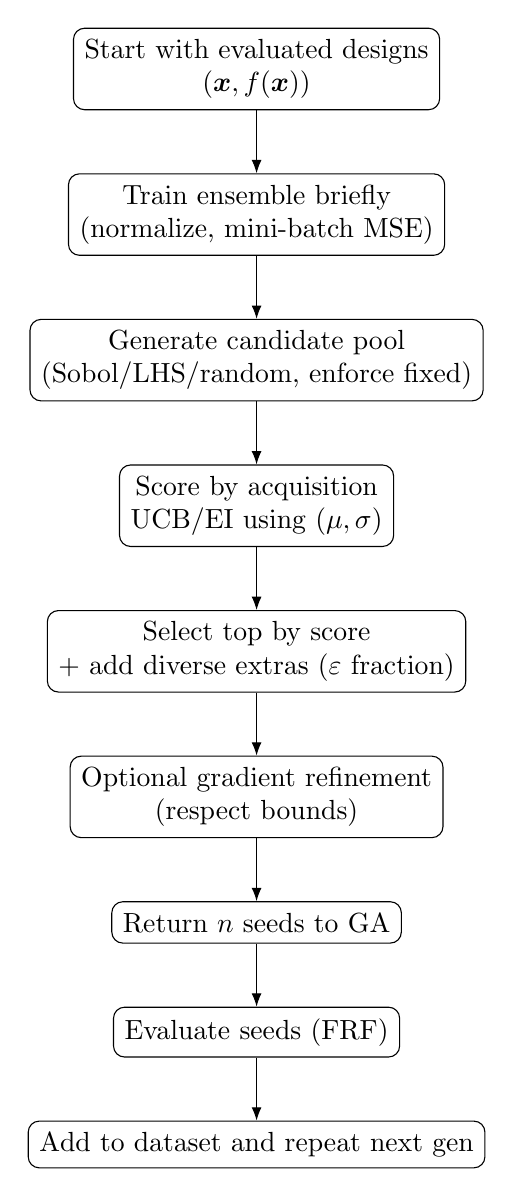
\begin{tikzpicture}[node distance=10mm, line/.style={-Latex}, box/.style={rectangle,draw,rounded corners,inner sep=4pt,align=center}]
\node[box] (data) {Start with evaluated designs\\$(\bm{x},f(\bm{x}))$};
\node[box,below=8mm of data] (train) {Train ensemble briefly\\(normalize, mini-batch MSE)};
\node[box,below=8mm of train] (pool) {Generate candidate pool\\(Sobol/LHS/random, enforce fixed)};
\node[box,below=8mm of pool] (score) {Score by acquisition\\UCB/EI using $(\mu,\sigma)$};
\node[box,below=8mm of score] (select) {Select top by score\\+ add diverse extras ($\varepsilon$ fraction)};
\node[box,below=8mm of select] (refine) {Optional gradient refinement\\(respect bounds)};
\node[box,below=8mm of refine] (seed) {Return $n$ seeds to GA};
\node[box,below=8mm of seed] (eval) {Evaluate seeds (FRF)};
\node[box,below=8mm of eval] (loop) {Add to dataset and repeat next gen};
\draw[line] (data) -- (train);
\draw[line] (train) -- (pool);
\draw[line] (pool) -- (score);
\draw[line] (score) -- (select);
\draw[line] (select) -- (refine);
\draw[line] (refine) -- (seed);
\draw[line] (seed) -- (eval);
\draw[line] (eval) -- (loop);
\end{tikzpicture}
\end{center}

\paragraph{When to use which seeding method?}
\begin{itemize}
\item Use \textbf{Random} for quick tests or low dimensions.
\item Use \textbf{Sobol/LHS} for broad, even coverage when you have no prior data.
\item Use \textbf{Memory} to leverage previous runs or restart from good regions.
\item Use \textbf{Best-of-pool} when you can afford a larger initial screening and want both quality and spread.
\item Use \textbf{Neural} when evaluations are costly and you want the GA to start with informed, high-quality candidates that balance exploration and exploitation.
\end{itemize}






\section{Evolutionary Operators}

\subsection{Tournament Selection}
\textbf{Mathematical Formulation:}
For tournament size $k=3$, the selection probability for individual $i$ is:
\begin{equation}
P(\text{select } i) = \prod_{j \neq i} P(\text{win against } j) \label{eq:tournament_selection}
\end{equation}
where $P(\text{win against } j) = 1$ if $f_i < f_j$, $0.5$ if $f_i = f_j$, and $0$ if $f_i > f_j$.

\textbf{Implementation Details:}
\begin{enumerate}
\item Uses \texttt{tools.selTournament} from DEAP library for efficient tournament implementation
\item Tournament size $k$ is configurable (default: 3 competitors per tournament)
\item Designed for minimization fitness: lower fitness values have higher probability of winning
\item Computational complexity: $O(k \cdot |\mathcal{P}|)$ per generation, linear in population size
\end{enumerate}

\textbf{Parameter Explanations:}
\begin{itemize}
\item $k$: Number of individuals competing in each tournament (tournament size)
\item $P(\text{win against } j)$: Probability that individual $i$ wins against individual $j$
\item $\mathcal{P}$: Current population containing all candidate solutions
\item $f_i, f_j$: Fitness values of individuals $i$ and $j$ (lower values are better for minimization)
\end{itemize}

\subsection{Blend Crossover (BLX-$\alpha$)}
\textbf{Mathematical Formulation:}
For two parents $\bm{x} = (x_1, \dots, x_d)$ and $\bm{y} = (y_1, \dots, y_d)$:
\begin{enumerate}
\item For each gene $i$:
\begin{align}
d_i &= |x_i - y_i| \label{eq:blx_distance} \\
I_i &= [\min(x_i, y_i) - \alpha d_i, \max(x_i, y_i) + \alpha d_i] \label{eq:blx_interval}
\end{align}
where $\alpha = 0.5$ (blend factor)

\item Sample offspring gene:
\begin{equation}
x'_i \sim \mathcal{U}(I_i) \label{eq:blx_sampling}
\end{equation}

\item Apply bounds and fixed parameters:
\begin{equation}
x'_i = \begin{cases}
c_i & \text{if } i \in \mathcal{F} \\
\max(\ell_i, \min(x'_i, u_i)) & \text{otherwise}
\end{cases} \label{eq:blx_bounds}
\end{equation}
\end{enumerate}

\textbf{Implementation Details:}
\begin{enumerate}
\item Uses \texttt{tools.cxBlend} from DEAP with blend factor $\alpha=0.5$ for balanced exploration
\item Creates two offspring per parent pair, maintaining population size
\item Automatically handles parameter bound constraints to keep solutions feasible
\item Fixed parameters are enforced exactly and never modified during crossover
\item Blend factor $\alpha$ controls the balance between exploration (larger $\alpha$) and exploitation (smaller $\alpha$)
\end{enumerate}

\textbf{Parameter Explanations:}
\begin{itemize}
\item $\bm{x}, \bm{y}$: Two parent solutions selected for crossover
\item $\alpha$: Blend factor controlling how far beyond parent values the offspring can be generated
\item $d_i = |x_i - y_i|$: Absolute difference between parents for parameter $i$
\item $I_i$: Extended interval around parent values where offspring values are sampled
\item $\mathcal{U}(I_i)$: Uniform distribution over the interval $I_i$ for generating offspring values
\item $\ell_i, u_i$: Original parameter bounds that must be respected
\end{itemize}

\subsection{Dynamic Mutation with Bounds}
\textbf{Mathematical Formulation:}
For individual $\bm{x}$ and mutation probability $p_{\text{mut}}$:

\begin{enumerate}
\item Individual-level mutation decision:
\begin{equation}
\text{mutate} \sim \text{Bernoulli}(p_{\text{mut}}) \label{eq:mutation_decision}
\end{equation}

\item If mutate = True, for each gene $i \notin \mathcal{F}$:
\begin{equation}
\text{mutate gene } i \sim \text{Bernoulli}(p_{\text{ind}}) \label{eq:gene_mutation_decision}
\end{equation}

\item If gene $i$ selected for mutation:
\begin{align}
\Delta_i &= u_i - \ell_i \label{eq:parameter_range} \\
\delta_i &\sim \mathcal{U}(-\eta \Delta_i, \eta \Delta_i) \label{eq:mutation_perturbation} \\
x'_i &= x_i + \delta_i \label{eq:mutation_application}
\end{align}

\item Apply bounds:
\begin{equation}
x'_i = \max(\ell_i, \min(x'_i, u_i)) \label{eq:mutation_bounds}
\end{equation}
\end{enumerate}

\textbf{Adaptive Mutation Scale:}
The mutation scale $\eta$ adapts based on diversity and success:
\begin{equation}
\eta_{t+1} = \begin{cases}
\min(\eta_{\max}, \eta_t \cdot 1.25) & \text{if diversity } D < D_{\text{target}} \\
\max(\eta_{\min}, \eta_t \cdot 0.90) & \text{if diversity } D > D_{\text{target}} \\
\eta_t & \text{otherwise}
\end{cases} \label{eq:adaptive_mutation_scale}
\end{equation}

\textbf{Implementation Details:}
\begin{enumerate}
\item Gene-level mutation probability $p_{\text{ind}} = 0.1$ (10\% chance per gene when individual is selected for mutation)
\item Dynamic mutation scale bounds: $\eta_{\min} = 0.01$, $\eta_{\max} = 0.30$ to prevent too small or too large perturbations
\item Fixed parameters are never mutated to maintain design constraints
\item Parameter bounds are enforced after mutation to keep solutions feasible
\item Mutation scale adapts every generation based on population diversity metrics
\end{enumerate}

\textbf{Parameter Explanations:}
\begin{itemize}
\item $p_{\text{mut}}$: Probability that an individual will undergo mutation (individual-level decision)
\item $p_{\text{ind}}$: Probability that each gene will be mutated when the individual is selected for mutation
\item $\eta$: Mutation scale factor controlling the magnitude of random perturbations
\item $\Delta_i = u_i - \ell_i$: Range of parameter $i$ used to scale the mutation magnitude
\item $\mathcal{N}(0, \sigma_i^2)$: Normal distribution centered at zero with parameter-specific variance
\item $D_{\text{target}}$: Target diversity level that the adaptive mechanism tries to maintain
\item $\eta_{\min}, \eta_{\max}$: Minimum and maximum allowed mutation scale values
\end{itemize}

\subsection{Elitism and Population Replacement}
\textbf{Mathematical Formulation:}
The offspring population $\mathcal{O}$ replaces the parent population $\mathcal{P}$:
\begin{equation}
\mathcal{P}_{t+1} = \mathcal{O}_t \label{eq:generational_replacement}
\end{equation}
where $\mathcal{O}_t$ contains all offspring from selection, crossover, and mutation.

\textbf{Optional Elitism:}
\begin{equation}
\mathcal{P}_{t+1} = \text{selBest}(\mathcal{P}_t \cup \mathcal{O}_t, |\mathcal{P}|) \label{eq:elitist_replacement}
\end{equation}

\textbf{Implementation Details:}
\begin{enumerate}
\item Standard generational replacement: offspring completely replace parent population
\item No elitism by default (can be configured to preserve best individuals)
\item Population size remains constant throughout evolution
\item All offspring are evaluated before replacing the parent population
\end{enumerate}

\textbf{Parameter Explanations:}
\begin{itemize}
\item $\mathcal{P}_t$: Parent population at generation $t$
\item $\mathcal{O}_t$: Offspring population generated from parents through selection, crossover, and mutation
\item $\text{selBest}(\cdot, k)$: Function that selects the $k$ best individuals by fitness
\item $|\mathcal{P}|$: Population size (constant throughout evolution)
\end{itemize}

\begin{algorithm}[H]
\caption{One Generation (selection, crossover, mutation, repair)}
\begin{algorithmic}[1]
\State $\mathcal{O} \leftarrow$ clone(\textsc{SelectTournament}$(\mathcal{P},|\mathcal{P}|,t=3)$)
\ForAll{pairs $(o_1,o_2) \in \mathcal{O}$}
\If{\textsc{Rand}() $< p_{\text{cx}}$} \State $(o_1,o_2) \leftarrow$ \textsc{Blend}$(o_1,o_2,\beta)$; repair to bounds, apply fixed \EndIf
\EndFor
\ForAll{$o\in\mathcal{O}$}
\If{\textsc{Rand}() $< p_{\text{mut}}$} \State $o\leftarrow$ \textsc{Mutate}$(o,\eta)$; repair to bounds, apply fixed \EndIf
\EndFor
\State evaluate invalid $o\in\mathcal{O}$ using Algorithm~\ref{alg:evaluate}
\State replace $\mathcal{P}\leftarrow\mathcal{O}$
\end{algorithmic}
\end{algorithm}

\section{Fitness Evaluation}
\begin{algorithm}[H]
\caption{EvaluateIndividual($\bm{x}$)}\label{alg:evaluate}
\begin{algorithmic}[1]
\If{paused/aborted} \State \Return large penalty \EndIf
\State $s \leftarrow$ \textsc{FRF}$(\bm{x};\Theta,\Omega)$; if missing, sum composite measures
\State $f_1\leftarrow |s-1|$; $f_2\leftarrow \alpha\sum_i |x_i|$
\State $E\leftarrow \sum_{m}\sum_{k} |\Delta_{m,k}(\bm{x})|$
\State \Return $f(\bm{x}) = f_1 + f_2 + E/S$
\end{algorithmic}
\end{algorithm}

\section{Adaptive Hyperparameter Control}

\subsection{Controller Architecture}
The GAWorker implements three adaptive controller types for dynamic hyperparameter tuning:

\begin{enumerate}
\item \textbf{Legacy Heuristic}: Rule-based adaptation using success rate and diversity metrics
\item \textbf{ML Bandit Controller}: Multi-armed bandit using Upper Confidence Bound (UCB) algorithm
\item \textbf{RL Controller}: Reinforcement learning using Q-learning with epsilon-greedy exploration
\end{enumerate}

Each controller adapts crossover probability $p_{\text{cx}}$, mutation probability $p_{\text{mut}}$, and optionally population size $N$.

\subsection{Legacy Heuristic Controller}
\textbf{Success Rate Tracking:}
Exponential Moving Average (EMA) of success rate:
\begin{equation}
\hat{s}_t = \alpha_s \cdot s_t + (1 - \alpha_s) \cdot \hat{s}_{t-1} \label{eq:success_rate_ema}
\end{equation}
where $s_t$ is current generation success rate, $\alpha_s = 0.20$ (smoothing factor).

\textbf{Diversity Tracking:}
EMA of gene-level diversity:
\begin{equation}
\hat{D}_t = \alpha_d \cdot D_t + (1 - \alpha_d) \cdot \hat{D}_{t-1} \label{eq:diversity_ema}
\end{equation}
where $D_t$ is current generation diversity, $\alpha_d = 0.20$.

\textbf{Adaptation Rules:}
\begin{align}
&\text{if } \hat{s}_t < 0.9 \cdot s^*:\; p_{\text{mut}} \leftarrow \min(\bar{p}_{\text{mut}},\, 1.25 \cdot p_{\text{mut}}) \quad \text{(increase exploration)} \label{eq:heuristic_low_success} \\
&\text{if } \hat{s}_t > 1.1 \cdot s^*:\; p_{\text{mut}} \leftarrow \max(\underline{p}_{\text{mut}},\, 0.8 \cdot p_{\text{mut}}) \quad \text{(decrease exploration)} \label{eq:heuristic_high_success} \\
&\text{if } \hat{D}_t < 0.08:\; p_{\text{mut}} \leftarrow \min(\bar{p}_{\text{mut}},\, 1.35 \cdot p_{\text{mut}}), \notag \\
&\quad \quad \quad \quad \quad p_{\text{cx}} \leftarrow \max(\underline{p}_{\text{cx}},\, 0.90 \cdot p_{\text{cx}}), \notag \\
&\quad \quad \quad \quad \quad \eta \leftarrow \min(\eta_{\max},\, 1.25 \cdot \eta) \quad \text{(boost exploration)} \label{eq:heuristic_low_diversity} \\
&\text{if } \hat{D}_t > 0.35:\; p_{\text{cx}} \leftarrow \min(\bar{p}_{\text{cx}},\, 1.20 \cdot p_{\text{cx}}), \notag \\
&\quad \quad \quad \quad \quad p_{\text{mut}} \leftarrow \max(\underline{p}_{\text{mut}},\, 0.90 \cdot p_{\text{mut}}), \notag \\
&\quad \quad \quad \quad \quad \eta \leftarrow \max(\eta_{\min},\, 0.90 \cdot \eta) \quad \text{(boost exploitation)} \label{eq:heuristic_high_diversity}
\end{align}

\textbf{Stagnation Detection:}
\begin{equation}
\text{stagnation\_counter} \leftarrow \begin{cases}
0 & \text{if improved this generation} \\
\text{stagnation\_counter} + 1 & \text{otherwise}
\end{cases} \label{eq:stagnation_detection}
\end{equation}

\subsection{ML Bandit Controller (Upper Confidence Bound)}
\textbf{Action Space:}
Discrete actions for parameter adjustments:
\begin{equation}
\mathcal{A} = \{(\delta_{cx}, \delta_{mut}, \rho) \mid \delta_{cx},\delta_{mut} \in \{-0.30,-0.15,0,0.15,0.30\}, \rho \in \{0.75,1.0,1.25\}\} \label{eq:bandit_action_space}
\end{equation}

\textbf{Per-Action Statistics:}
For each action $a \in \mathcal{A}$:
\begin{itemize}
\item Count: $n_a$ (times action selected)
\item Average reward: $\bar{R}_a = \frac{1}{n_a} \sum_{i=1}^{n_a} R_a^{(i)}$
\end{itemize}

\textbf{UCB Selection:}
At time step $t$ (total action selections):
\begin{equation}
a_t = \arg\max_{a \in \mathcal{A}} \left[ w_h \cdot \bar{R}_a + w_c \cdot R_t + c \cdot \sqrt{\frac{\ln t}{n_a}} \right] \label{eq:ucb_selection}
\end{equation}
where:
\begin{itemize}
\item $w_h = 0.7$ (historical weight)
\item $w_c = 0.3$ (current weight)
\item $c = 0.6$ (exploration parameter)
\end{itemize}

\textbf{Reward Function:}
\begin{equation}
R_t = \frac{\max(0, f_{t-1}^* - f_t^*)}{\max(\Delta t, \epsilon) \cdot \max(\#\text{evals}_t, 1)} - \lambda \cdot |cv_t - cv^*| \label{eq:bandit_reward}
\end{equation}
where:
\begin{itemize}
\item $f_t^*$ is best fitness in generation $t$
\item $\Delta t$ is generation time
\item $\#$evals$_t$ is number of evaluations in generation $t$
\item $\lambda = 0.02$ (diversity penalty weight)
\item $cv^*$ = 0.2 (target coefficient of variation)
\end{itemize}

\textbf{Parameter Application:}
After selecting action $(\delta_{cx}, \delta_{mut}, \rho)$:
\begin{align}
p_{\text{cx}} &\leftarrow \max(\underline{p}_{\text{cx}}, \min(\bar{p}_{\text{cx}}, p_{\text{cx}} \cdot (1 + \delta_{cx}))) \label{eq:bandit_cx_update} \\
p_{\text{mut}} &\leftarrow \max(\underline{p}_{\text{mut}}, \min(\bar{p}_{\text{mut}}, p_{\text{mut}} \cdot (1 + \delta_{mut}))) \label{eq:bandit_mut_update} \\
N &\leftarrow \max(N_{\min}, \min(N_{\max}, \lfloor N \cdot \rho \rfloor)) \label{eq:bandit_pop_update}
\end{align}

\subsection{Reinforcement Learning Controller}
\textbf{State Space:}
Simple state encoding based on progress:
\begin{equation}
s_t = \begin{cases}
0 & \text{if } f_t^* < f_{t-1}^* \text{ (improvement)} \\
1 & \text{if } f_t^* \geq f_{t-1}^* \text{ (no improvement)}
\end{cases} \label{eq:rl_state}
\end{equation}

\textbf{Q-Table:}
Tabular Q-values for state-action pairs:
\begin{equation}
Q(s,a) \quad \forall s \in \{0,1\}, a \in \mathcal{A} \label{eq:q_table}
\end{equation}
Initialized to zeros.

\textbf{Epsilon-Greedy Action Selection:}
\begin{equation}
a_t = \begin{cases}
\arg\max_{a} Q(s_t, a) & \text{with probability } 1 - \varepsilon_t \\
\text{random } a \in \mathcal{A} & \text{with probability } \varepsilon_t
\end{cases} \label{eq:epsilon_greedy}
\end{equation}

\textbf{Epsilon Decay:}
\begin{equation}
\varepsilon_{t+1} = \varepsilon_t \cdot \varepsilon_{\text{decay}} \label{eq:epsilon_decay}
\end{equation}
with $\varepsilon_{\text{decay}} = 0.95$.

\textbf{Q-Learning Update:}
After observing reward $R_t$ and next state $s_{t+1}$:
\begin{equation}
Q(s_t, a_t) \leftarrow Q(s_t, a_t) + \alpha \left[ R_t + \gamma \max_{a'} Q(s_{t+1}, a') - Q(s_t, a_t) \right] \label{eq:q_learning_update}
\end{equation}
where $\alpha = 0.1$ (learning rate), $\gamma = 0.9$ (discount factor).

\textbf{RL Reward Shaping:}
\begin{equation}
R_t = w_1 \cdot \frac{\max(0, f_{t-1}^* - f_t^*)}{1 + |f_t^*|} + w_2 \cdot \frac{D_t - D_{t-1}}{1 + D_{t-1}} + w_3 \cdot \frac{1}{\max(\Delta t, \epsilon)} - w_4 \cdot |cv_t - cv^*| \label{eq:rl_reward_shaping}
\end{equation}
where:
\begin{itemize}
\item $w_1 = 1.0$ (improvement weight)
\item $w_2 = 0.0$ (diversity weight)
\item $w_3 = 0.0$ (speed weight)
\item $w_4 = 0.02$ (diversity penalty weight)
\end{itemize}
\subsection{Surrogate-Assisted Screening}
\textbf{Surrogate Model Architecture:}
\textbf{Normalization and Distance Metric:}
GAWorker normalizes all parameter vectors to the unit hypercube $[0,1]^d$:
\begin{equation}
\tilde{x}_i = \frac{x_i - \ell_i}{u_i - \ell_i} \label{eq:surrogate_normalization}
\end{equation}
where $\ell_i$ and $u_i$ are the parameter bounds.

\textbf{k-Nearest Neighbors Prediction:}
For a candidate solution $\bm{z}$, compute Euclidean distances to all archived points:
\begin{equation}
d_j(\bm{z}) = \sqrt{\sum_{i=1}^d (\tilde{z}_i - \tilde{x}_i^{(j)})^2} \quad \forall j = 1, \dots, m \label{eq:surrogate_distance}
\end{equation}
where $m$ is the size of the archive.

Select $k$ nearest neighbors $\mathcal{N}_k(\bm{z})$ and predict fitness:
\begin{equation}
\hat{f}(\bm{z}) = \frac{1}{k} \sum_{j \in \mathcal{N}_k(\bm{z})} f(\bm{x}^{(j)}) \label{eq:surrogate_prediction}
\end{equation}

\textbf{Weighted kNN Variant:}
Distance-weighted prediction for improved accuracy:
\begin{equation}
\hat{f}(\bm{z}) = \frac{\sum_{j \in \mathcal{N}_k(\bm{z})} w_j \cdot f(\bm{x}^{(j)})}{\sum_{j \in \mathcal{N}_k(\bm{z})} w_j} \label{eq:weighted_surrogate}
\end{equation}
where $w_j = \frac{1}{d_j(\bm{z}) + \epsilon}$ is the inverse distance weight.

\subsection{RL controller (Q-learning)}
States $s\in\{0,1\}$ encode coarse progress; actions are as above. Epsilon-greedy selection and tabular update
\[ Q(s,a) \leftarrow Q(s,a) + \alpha\,\big[ r + \gamma \max_{a'} Q(s',a') - Q(s,a)\big]. \]
\begin{algorithm}[H]
\caption{RL step}
\begin{algorithmic}[1]
\State with prob. $\varepsilon$ pick random $a$, else $\arg\max_a Q(s,a)$
\State apply $a$, run generation, observe reward $r$ and next state $s'$
\State $Q(s,a)\leftarrow Q(s,a)+\alpha\,[r+\gamma\max_{a'}Q(s',a')-Q(s,a)]$
\State $s\leftarrow s'$, $\varepsilon\leftarrow \varepsilon\cdot\text{decay}$
\end{algorithmic}
\end{algorithm}

\paragraph{Controller decision tree.}
\begin{center}
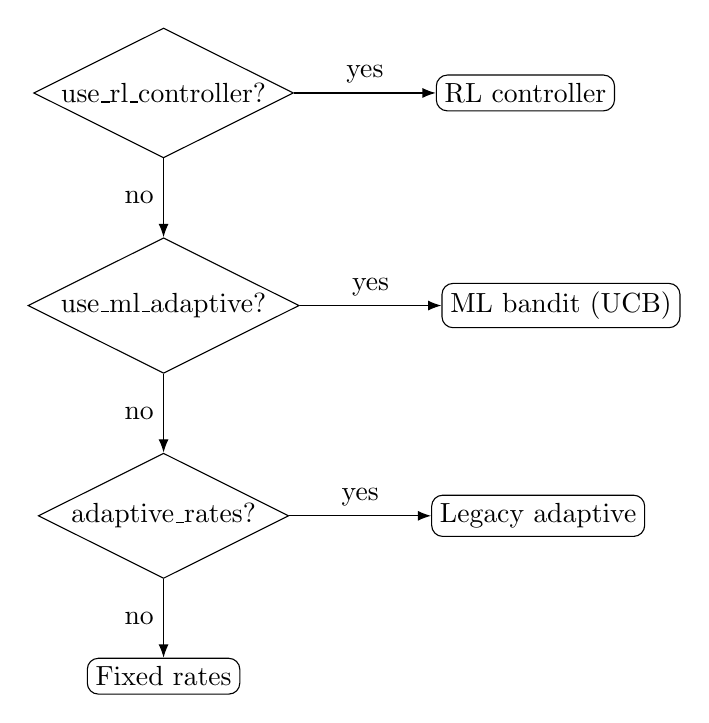
\begin{tikzpicture}[node distance=10mm, line/.style={-Latex}, decision/.style={diamond,draw,aspect=2,inner sep=1pt,align=center}, block/.style={rectangle,draw,rounded corners,inner sep=3pt,align=center}]
\node[decision] (rl) {use\_rl\_controller?};
\node[block,right=18mm of rl] (rlb) {RL controller};
\draw[line] (rl) -- node[above]{yes} (rlb);
\node[decision,below=10mm of rl] (ml) {use\_ml\_adaptive?};
\draw[line] (rl) -- node[left]{no} (ml);
\node[block,right=18mm of ml] (mlb) {ML bandit (UCB)};
\draw[line] (ml) -- node[above]{yes} (mlb);
\node[decision,below=10mm of ml] (adp) {adaptive\_rates?};
\draw[line] (ml) -- node[left]{no} (adp);
\node[block,right=18mm of adp] (adpb) {Legacy adaptive};
\node[block,below=10mm of adp] (fix) {Fixed rates};
\draw[line] (adp) -- node[above]{yes} (adpb);
\draw[line] (adp) -- node[left]{no} (fix);
\end{tikzpicture}
\end{center}

\section{Statistical Analysis and Visualization Methods}

\subsection{Parameter Sensitivity Analysis}
GAWorker includes comprehensive statistical analysis methods for understanding parameter effects and optimization results.

\subsubsection{Parameter Distribution Analysis}
For each parameter $x_i$ across a set of solutions $\mathcal{S} = \{\bm{x}^{(1)}, \dots, \bm{x}^{(N)}\}$:

\textbf{Descriptive Statistics:}
\begin{align}
\text{mean}_i &= \frac{1}{N} \sum_{j=1}^N x_i^{(j)} \label{eq:parameter_mean} \\
\text{std}_i &= \sqrt{\frac{1}{N-1} \sum_{j=1}^N (x_i^{(j)} - \text{mean}_i)^2} \label{eq:parameter_std} \\
\text{skewness}_i &= \frac{\frac{1}{N} \sum_{j=1}^N (x_i^{(j)} - \text{mean}_i)^3}{\text{std}_i^3} \label{eq:parameter_skewness} \\
\text{kurtosis}_i &= \frac{\frac{1}{N} \sum_{j=1}^N (x_i^{(j)} - \text{mean}_i)^4}{\text{std}_i^4} - 3 \label{eq:parameter_kurtosis}
\end{align}

\subsubsection{Distribution Fitting and Normality Tests}
\textbf{Shapiro-Wilk Test for Normality:}
\begin{equation}
W = \frac{\left(\sum_{i=1}^n a_i x_{(i)}\right)^2}{\sum_{i=1}^n (x_i - \bar{x})^2} \label{eq:shapiro_wilk}
\end{equation}
where $x_{(i)}$ are ordered statistics and $a_i$ are tabulated coefficients.

\textbf{Anderson-Darling Test:}
\begin{equation}
A^2 = -n - \frac{1}{n} \sum_{i=1}^n (2i-1) \left[\ln F_0(x_{(i)}) + \ln(1 - F_0(x_{(n+1-i)}))\right] \label{eq:anderson_darling}
\end{equation}

\subsubsection{Parameter Correlation Analysis}
\textbf{Pearson Correlation Coefficient:}
\begin{equation}
r_{ij} = \frac{\sum_{k=1}^N (x_i^{(k)} - \bar{x}_i)(x_j^{(k)} - \bar{x}_j)}{\sqrt{\sum_{k=1}^N (x_i^{(k)} - \bar{x}_i)^2} \sqrt{\sum_{k=1}^N (x_j^{(k)} - \bar{x}_j)^2}} \label{eq:pearson_correlation}
\end{equation}

\textbf{Spearman Rank Correlation:}
\begin{equation}
\rho_{ij} = 1 - \frac{6 \sum_{k=1}^N d_k^2}{N(N^2 - 1)} \label{eq:spearman_correlation}
\end{equation}
where $d_k$ is the difference between ranks for observation $k$.

\subsubsection{Parameter Importance Ranking}
\textbf{Variance Inflation Factor (VIF):}
\begin{equation}
\text{VIF}_i = \frac{1}{1 - R_i^2} \label{eq:vif}
\end{equation}
where $R_i^2$ is the coefficient of determination from regressing $x_i$ on all other parameters.

\textbf{Principal Component Analysis (PCA):}
For parameter matrix $\mathbf{X} \in \mathbb{R}^{N \times d}$:
\begin{enumerate}
\item Standardize: $\mathbf{X}' = (\mathbf{X} - \bm{\mu}) \mathbf{\Sigma}^{-1/2}$
\item Compute covariance: $\mathbf{C} = \frac{1}{N-1} \mathbf{X}'^\top \mathbf{X}'$
\item Eigenvalue decomposition: $\mathbf{C} = \mathbf{V} \mathbf{\Lambda} \mathbf{V}^\top$
\item Explained variance ratio: $\frac{\lambda_j}{\sum_{k=1}^d \lambda_k}$
\end{enumerate}

\subsection{Random Validation and Monte Carlo Analysis}
\textbf{Implementation:}
The system supports Monte Carlo validation with multiple sampling methods:

\subsubsection{Sampling Methods}
\begin{enumerate}
\item \textbf{Random Uniform:} $x_i \sim \mathcal{U}(\ell_i, u_i)$
\item \textbf{Latin Hypercube:} Stratified sampling ensuring coverage
\item \textbf{Sobol Sequences:} Low-discrepancy quasi-random sampling
\item \textbf{Monte Carlo with Importance Sampling:} $x_i \sim p(x_i | \text{importance})$
\end{enumerate}

\subsubsection{Convergence Metrics}
\textbf{Monte Carlo Error Estimation:}
\begin{equation}
\sigma_{\text{MC}} = \sqrt{\frac{1}{N(N-1)} \sum_{i=1}^N (f_i - \bar{f})^2} \label{eq:monte_carlo_error}
\end{equation}

\textbf{Confidence Intervals:}
\begin{equation}
\bar{f} \pm t_{\alpha/2, N-1} \cdot \frac{\sigma_{\text{MC}}}{\sqrt{N}} \label{eq:confidence_intervals}
\end{equation}

\subsection{Benchmarking and Performance Metrics}
\subsubsection{Computational Performance Tracking}
\textbf{CPU Utilization:}
\begin{equation}
\text{CPU\%}_t = \frac{\text{CPU time used}}{\text{total elapsed time}} \times 100 \label{eq:cpu_utilization}
\end{equation}

\textbf{Memory Usage:}
\begin{equation}
\text{Memory (MB)} = \frac{\text{RSS bytes}}{1024 \times 1024} \label{eq:memory_usage}
\end{equation}

\subsubsection{Algorithm Efficiency Metrics}
\textbf{Evaluations per Second:}
\begin{equation}
\text{EPS} = \frac{\text{total evaluations}}{\text{total time (seconds)}} \label{eq:evaluations_per_second}
\end{equation}

\textbf{Improvement Rate:}
\begin{equation}
\text{IR}_t = \frac{f^*_{t-1} - f^*_t}{\Delta t} \label{eq:improvement_rate}
\end{equation}

\subsubsection{Statistical Significance Testing}
\textbf{Wilcoxon Signed-Rank Test:}
For comparing algorithm performance across runs:
\begin{equation}
W = \sum_{i=1}^n \text{rank}(|d_i|) \cdot \text{sign}(d_i) \label{eq:wilcoxon_test}
\end{equation}
where $d_i = f_{A,i} - f_{B,i}$ are paired differences.

\subsubsection{Parameter Range Recommendations}
\textbf{Interquartile Range (IQR) Method:}
\begin{align}
\text{IQR} &= Q_3 - Q_1 \label{eq:iqr_calculation} \\
\text{Recommended range} &= [Q_1 - 1.5 \cdot \text{IQR}, Q_3 + 1.5 \cdot \text{IQR}] \label{eq:iqr_range}
\end{align}

\textbf{Percentile-Based Ranges:}
\begin{equation}
\text{P5-P95 range} = [P_5, P_{95}] \label{eq:percentile_range}
\end{equation}

\textbf{Statistical Distribution Fitting:}
The system fits multiple distributions and selects the best using:
\begin{align}
\text{AIC} &= 2k - 2\ln(\hat{L}) \label{eq:aic_criterion} \\
\text{BIC} &= k \ln(n) - 2\ln(\hat{L}) \label{eq:bic_criterion}
\end{align}

\textbf{Parameter Explanations:}
\begin{itemize}
\item $Q_1, Q_3$: First and third quartiles (25th and 75th percentiles) of the parameter values
\item $\text{IQR} = Q_3 - Q_1$: Interquartile range measuring the spread of the middle 50\% of data
\item $P_5, P_{95}$: 5th and 95th percentiles, capturing the central 90\% of the distribution
\item $k$: Number of parameters in the statistical model being fitted
\item $n$: Number of data points used for fitting the distribution
\item $\hat{L}$: Maximum likelihood estimate of the data given the fitted distribution
\end{itemize}

\subsection{Visualization Methods}
\subsubsection{Advanced Plot Types}
\begin{enumerate}
\item \textbf{Violin Plots:} Show parameter distributions with kernel density estimation
\item \textbf{Box Plots:} Display quartiles and outliers
\item \textbf{Histograms:} Frequency distributions with fitted curves
\item \textbf{Q-Q Plots:} Quantile-quantile comparisons for distribution fitting
\item \textbf{Scatter Matrix:} Pairwise parameter relationships
\item \textbf{Correlation Heatmaps:} Parameter correlation matrices
\item \textbf{Parallel Coordinates:} Multi-dimensional parameter visualization
\end{enumerate}

\subsubsection{Interactive Analysis Features}
\begin{itemize}
\item Parameter selection and filtering
\item Statistical summary tables
\item Export capabilities (CSV, JSON, images)
\item Real-time visualization updates
\item Comparative analysis across runs
\end{itemize}

\section{Surrogate-Assisted Screening}
When the genetic algorithm (GA) produces new offspring that have not yet been evaluated (i.e., "invalid" individuals), and there is a sufficiently large history of past evaluated solutions, the GAWorker uses a surrogate-assisted screening process to decide which candidates to actually evaluate with the expensive objective function. This process is designed to save computation by focusing evaluations on the most promising or diverse candidates.

\subsection{Surrogate Model Architecture}
\textbf{Normalization and Distance Metric:}
GAWorker normalizes all parameter vectors to the unit hypercube $[0,1]^d$:
\[
\tilde{x}_i = \frac{x_i - \ell_i}{u_i - \ell_i}
\]
where $\ell_i$ and $u_i$ are the parameter bounds.

\textbf{k-Nearest Neighbors Prediction:}
For a candidate solution $\bm{z}$, compute Euclidean distances to all archived points:
\[
d_j(\bm{z}) = \sqrt{\sum_{i=1}^d (\tilde{z}_i - \tilde{x}_i^{(j)})^2} \quad \forall j = 1, \dots, m
\]
where $m$ is the size of the archive.

Select $k$ nearest neighbors $\mathcal{N}_k(\bm{z})$ and predict fitness:
\[
\hat{f}(\bm{z}) = \frac{1}{k} \sum_{j \in \mathcal{N}_k(\bm{z})} f(\bm{x}^{(j)})
\]

\textbf{Weighted kNN Variant:}
Distance-weighted prediction for improved accuracy:
\[
\hat{f}(\bm{z}) = \frac{\sum_{j \in \mathcal{N}_k(\bm{z})} w_j \cdot f(\bm{x}^{(j)})}{\sum_{j \in \mathcal{N}_k(\bm{z})} w_j}
\]
where $w_j = \frac{1}{d_j(\bm{z}) + \epsilon}$ is the inverse distance weight.

\subsection{Screening Strategy}
\textbf{Pool Generation:}
Generate candidate pool $\mathcal{U}$ by evolutionary operations:
\begin{enumerate}
\item Start with current invalid offspring $\mathcal{I}$
\item Apply crossover and mutation to generate additional candidates
\item Ensure $|\mathcal{U}| = \lceil \rho \cdot |\mathcal{I}| \rceil$ where $\rho > 1$ is pool factor
\item Enforce parameter bounds and fixed constraints
\end{enumerate}

\textbf{Exploration vs Exploitation:}
Sort candidates by surrogate prediction: $\hat{f}^{(1)} \leq \hat{f}^{(2)} \leq \dots \leq \hat{f}^{(|\mathcal{U}|)}$

Select exploitation candidates:
\begin{equation}
\mathcal{E} = \{\bm{x}^{(j)} \mid j = 1, \dots, \lfloor (1-\xi) \cdot q \rfloor\} \label{eq:exploitation_selection}
\end{equation}

\textbf{Diversity-Based Exploration:}
For exploration candidates, compute novelty scores:
\begin{equation}
\text{novelty}(\bm{x}) = \min_{j=1,\dots,m} d_j(\bm{x}) \label{eq:novelty_score}
\end{equation}
Select most novel candidates:
\begin{equation}
\mathcal{X} = \text{top } \lceil \xi \cdot q \rceil \text{ by novelty}(\cdot) \label{eq:exploration_selection}
\end{equation}

\textbf{Final Selection:}
\begin{equation}
\mathcal{S} = \mathcal{E} \cup \mathcal{X}, \quad |\mathcal{S}| = q \label{eq:final_surrogate_selection}
\end{equation}

\textbf{Parameter Explanations:}
\begin{itemize}
\item $\mathcal{I}$: Set of invalid offspring that need fitness evaluation
\item $\rho$: Pool expansion factor (typically 2.0-3.0) to create larger candidate pool
\item $\mathcal{U}$: Expanded candidate pool for surrogate screening
\item $\xi$: Exploration fraction (typically 0.1-0.2) controlling balance between exploitation and exploration
\item $\mathcal{E}$: Exploitation set containing highest predicted fitness candidates
\item $\mathcal{X}$: Exploration set containing most novel candidates
\item $\mathcal{S}$: Final selected set of candidates that will receive true fitness evaluation
\end{itemize}

\subsection{Surrogate Quality Metrics}
\textbf{Prediction Error Tracking:}
Root Mean Square Error (RMSE):
\begin{equation}
\text{RMSE} = \sqrt{\frac{1}{|\mathcal{S}|} \sum_{\bm{x} \in \mathcal{S}} (\hat{f}(\bm{x}) - f(\bm{x}))^2} \label{eq:surrogate_rmse}
\end{equation}

\textbf{Rank Correlation:}
Spearman's $\rho$ between predicted and actual rankings:
\begin{equation}
\rho = 1 - \frac{6 \sum_{i=1}^q d_i^2}{q(q^2 - 1)} \label{eq:surrogate_rank_correlation}
\end{equation}
where $d_i$ is the difference between predicted and actual ranks.

\textbf{Surrogate Efficiency:}
Evaluations saved per generation:
\begin{equation}
\text{Efficiency} = \frac{|\mathcal{U}| - q}{|\mathcal{U}|} \times 100\% \label{eq:surrogate_efficiency}
\end{equation}

\textbf{Parameter Explanations:}
\begin{itemize}
\item $|\mathcal{S}|$: Number of candidates actually evaluated with true fitness function
\item $\hat{f}(\bm{x})$: Surrogate prediction of fitness for candidate $\bm{x}$
\item $f(\bm{x})$: True fitness value obtained from expensive evaluation
\item $q$: Target number of evaluations per generation (typically equals population size)
\item $d_i$: Distance between predicted and actual ranking positions for Spearman correlation
\end{itemize}

\textbf{Screening Procedure:}
\begin{itemize}
    \item \emph{Pool Construction:} GAWorker generates a pool of candidate offspring by applying crossover, mutation, and cloning until the pool size reaches $\lceil \rho q \rceil$, where $q$ is the number of evaluations to perform and $\rho > 1$ is a pool factor (e.g., 2).
    \item \emph{Surrogate Prediction:} For each candidate in the pool, the kNN surrogate predicts its fitness $\hat{f}$.
    \item \emph{Exploitation vs. Exploration:} The $q$ candidates to be evaluated are chosen as follows:
    \begin{itemize}
        \item A fraction $q_e = \lfloor (1-\xi)q \rfloor$ (where $\xi$ is the exploration fraction, e.g., 0.15) are selected with the lowest predicted $\hat{f}$ (i.e., most promising according to the surrogate).
        \item The remaining $q_x = q - q_e$ are selected for diversity: these are the candidates with the largest minimum distance to any point in the archive (i.e., most novel).
    \end{itemize}
    \item \emph{Evaluation and Replacement:} Only these $q$ selected candidates are evaluated with the true objective function, and their results are used to replace the invalid offspring in the population.
\end{itemize}

This surrogate screening strategy, as implemented in \texttt{GAWorker.py}, allows the algorithm to balance exploitation (focusing on candidates likely to improve the objective) and exploration (sampling novel regions of the search space), while reducing the number of expensive function evaluations per generation.

\begin{algorithm}[H]
\caption{Surrogate screening of invalid offspring}
\begin{algorithmic}[1]
\Require target evaluate count $q$, pool factor $\rho>1$, history $\{(\bm{x}^{(j)},y_j)\}$
\State build pool $\mathcal{U}$ by cloning/mutating/crossover until $|\mathcal{U}|=\lceil \rho q\rceil$
\State compute $\hat{f}(\cdot)$ by $k$NN in $[0,1]^d$; sort $\mathcal{U}$ ascending
\State $q_e\leftarrow \lfloor (1-\xi) q\rfloor$ exploit, $q_x\leftarrow q-q_e$ explore
\State choose first $q_e$ by lowest $\hat{f}$; choose $q_x$ by novelty (max min-distance)
\State evaluate chosen; replace invalid offspring accordingly
\end{algorithmic}
\end{algorithm}

\paragraph{Surrogate decision.}
\begin{center}
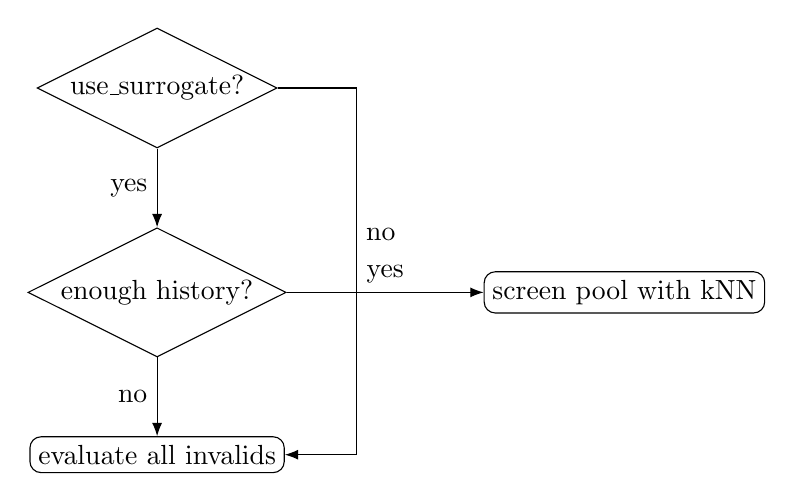
\begin{tikzpicture}[node distance=10mm, line/.style={-Latex}, decision/.style={diamond,draw,aspect=2,inner sep=1pt,align=center}, block/.style={rectangle,draw,rounded corners,inner sep=3pt,align=center}]
\node[decision] (use) {use\_surrogate?};
\node[decision,below=10mm of use] (enough) {enough history?};
\node[block,right=25mm of enough] (screen) {screen pool with kNN};
\node[block,below=10mm of enough] (eval) {evaluate all invalids};
\draw[line] (use) -- node[left]{yes} (enough);
\draw[line] (use.east) --++ (10mm,0) |- node[pos=.2,right]{no} (eval);
\draw[line] (enough) -- node[above]{yes} (screen);
\draw[line] (enough) -- node[left]{no} (eval);
\end{tikzpicture}
\end{center}

\section{Complete Algorithm}
\begin{algorithm}[H]
\caption{GAWorker main loop}
\begin{algorithmic}[1]
\State initialize seeding method and population $\mathcal{P}_0$ (Algorithm 1); evaluate all
\For{$t=1$ to $T$}
\State if paused/aborted: break
\State select controller by decision tree; update $(p_{\text{cx}},p_{\text{mut}},N)$; resize if needed
\State run one generation (selection, crossover, mutation, repair)
\State evaluate invalid offspring; if surrogate enabled and ready, screen first
\State update best-so-far, statistics $(\mu,\sigma,cv,D)$, success rate, EMAs
\State apply adaptive heuristics or controller updates; log metrics
\State if $\min f \le \varepsilon$: break
\EndFor
\State return best individual and full metrics; compute final FRF and report
\end{algorithmic}
\end{algorithm}

\textbf{Algorithm Parameter Explanations:}
\begin{itemize}
\item $\mathcal{P}_0$: Initial population created using the selected seeding method
\item $T$: Maximum number of generations (termination criterion)
\item $p_{\text{cx}}, p_{\text{mut}}$: Crossover and mutation probabilities (may be adaptive)
\item $N$: Population size (may change if adaptive population sizing is enabled)
\item $\mu, \sigma$: Population mean and standard deviation of fitness values
\item $cv$: Coefficient of variation measuring population diversity
\item $D$: Gene-level diversity metric across all parameters
\item $\varepsilon$: Convergence tolerance for early termination
\end{itemize}


\section{System Architecture and Implementation}

\subsection{Core Components Integration}
The GAWorker system integrates multiple sophisticated components:

\subsubsection{DEAP Framework Integration}
\textbf{Type Registration:}
\begin{enumerate}
\item \texttt{creator.create("FitnessMin", base.Fitness, weights=(-1.0,))}: Defines minimization fitness type
\item \texttt{creator.create("Individual", list, fitness=creator.FitnessMin)}: Creates individual representation
\item Custom toolbox registration for all genetic operators and evaluation functions
\end{enumerate}

\textbf{Framework Advantages:}
\begin{itemize}
\item Modular operator design allowing easy customization and extension
\item Built-in support for complex fitness functions and constraints
\item Efficient population management and statistics tracking
\item Seamless integration with Python scientific computing ecosystem
\end{itemize}

\subsubsection{PyQt5 Threading Architecture}
\textbf{Worker Thread Pattern:}
\begin{enumerate}
\item \texttt{QThread} inheritance enables non-blocking background execution
\item \texttt{pyqtSignal} provides thread-safe communication between worker and GUI
\item \texttt{QMutex} and \texttt{QWaitCondition} ensure proper synchronization
\end{enumerate}

\textbf{Threading Benefits:}
\begin{itemize}
\item GUI remains responsive during long optimization runs
\item Safe communication of progress updates and results
\item Ability to pause, resume, and cancel optimization processes
\item Proper resource cleanup and error handling
\end{itemize}

\subsubsection{PyTorch Neural Network Backend}
\textbf{Neural Seeder Architecture:}
\begin{enumerate}
\item Configurable network depth (layers) and width (neurons per layer)
\item Dropout regularization prevents overfitting during training
\item L2 weight decay encourages simpler models and better generalization
\item Time-capped training prevents excessive computation
\end{enumerate}

\textbf{Neural Network Features:}
\begin{itemize}
\item Automatic device selection (GPU if available, otherwise CPU)
\item Ensemble learning with multiple networks for uncertainty quantification
\item Gradient-based refinement for fine-tuning promising solutions
\item Incremental learning from new evaluation data
\end{itemize}

\subsection{Advanced Implementation Features}

\subsubsection{Robust Error Handling and Recovery}
\textbf{DEAP State Management:}
The system implements sophisticated error recovery:
\begin{itemize}
\item Automatic cleanup of DEAP global state on failures
\item Retry mechanisms with exponential backoff
\item Graceful degradation to simpler methods
\item Exception wrapping for user-friendly error messages
\end{itemize}

\subsubsection{Real-time System Monitoring}
\textbf{Performance Metrics Collection:}
\begin{itemize}
\item CPU utilization per core and system-wide
\item Memory usage (RSS, VMS, shared)
\item Disk I/O operations and data transfer
\item Network activity monitoring
\item Thread count and process information
\end{itemize}

\subsubsection{Memory Management and Optimization}
\textbf{Efficient Data Structures:}
\begin{itemize}
\item Numpy arrays for numerical computations
\item Pandas DataFrames for statistical analysis
\item JSON serialization for persistent storage
\item Lazy evaluation of expensive operations
\end{itemize}

\subsection{Configuration and Extensibility}

\subsubsection{JSON Configuration System}
The system uses hierarchical JSON configuration:
\begin{itemize}
\item Algorithm parameters (population size, rates, limits)
\item Controller settings (ML bandit, RL parameters)
\item Neural network architecture specifications
\item Statistical analysis options
\end{itemize}

\subsubsection{Plugin Architecture}
\textbf{Extensible Design:}
\begin{itemize}
\item Modular seeding methods
\item Interchangeable controllers
\item Pluggable statistical analyzers
\item Custom visualization backends
\end{itemize}

\section{Recommended Seeding–Surrogate–Adaptation Recipes}
\label{sec}
\begin{enumerate}

\item \textbf{LHS + kNN surrogate + ML–UCB}
\begin{itemize}
\item Seeding: \texttt{lhs}. Surrogate: \texttt{use\_surrogate=true}, \texttt{surrogate\_k=7}, \texttt{surrogate\_pool\_factor=2.5}, \texttt{surrogate\_explore\_frac=0.15}.
\item Adaptive: \texttt{use\_ml\_adaptive=true}, \texttt{ml\_ucb\_c=0.6}, \texttt{ml\_adapt\_population=true}, \texttt{pop\_min}, $\approx 0.75N$, \texttt{pop\_max}, $\approx 1.25N$.
\item Rationale: LHS provides stratified coverage that stabilizes kNN predictions; UCB balances exploration/exploitation with low regret, adapting rates and population to improve improvement-per-evaluation.
\end{itemize}

\item \textbf{Sobol + kNN surrogate (explorative) + heuristic adaptive rates}
\begin{itemize}
\item Seeding: \texttt{sobol}. Surrogate: \texttt{k=5}, \texttt{pool\_factor=2.0}, \texttt{explore\_frac=0.30}.
\item Adaptive: \texttt{adaptive\_rates=true}, \texttt{stagnation\_limit=5}, diversity-driven increase in mutation when coefficient of variation is low.
\item Rationale: Low-discrepancy Sobol seeds reduce initial clustering; higher surrogate exploration mitigates model bias on multimodal landscapes; diversity-based heuristics sustain global search.
\end{itemize}

\item \textbf{Memory seeding + kNN surrogate + RL controller}
\begin{itemize}
\item Seeding: \texttt{memory} (replay + jitter + explore). Surrogate: \texttt{k=5}, \texttt{pool\_factor=3.0}, \texttt{explore\_frac=0.20}.
\item Adaptive: \texttt{use\_rl\_controller=true}, \texttt{rl\_alpha=0.1}, \texttt{rl\_gamma=0.9}, \texttt{rl\_epsilon=0.2}, \texttt{rl\_epsilon\_decay=0.95}, \texttt{pop\_min}, $\approx 0.75N$, \texttt{pop\_max}, $\approx 1.25N$.
\item Rationale: Warm starts exploit prior data to cut cold-start cost; RL learns effective rate/pop moves from rewards shaped by improvement, time, and diversity, reducing wasted evaluations.
\end{itemize}

\item \textbf{Neural seeding (UCB, epsilon-adaptive) + kNN surrogate + ML–UCB}
\begin{itemize}
\item Seeding: \texttt{neural}, \texttt{neural\_acq\_type=ucb}, \texttt{neural\_adapt\_epsilon=true} (\texttt{eps\_min=0.05}, \texttt{eps\_max=0.30}), \texttt{neural\_pool\_mult=3.0}.
\item Surrogate: \texttt{k=5}, \texttt{pool\_factor=2.0}, \texttt{explore\_frac=0.15}. Adaptive: \texttt{use\_ml\_adaptive=true}, \texttt{ml\_ucb\_c=0.6}, \texttt{ml\_adapt\_population=true}.
\item Rationale: Model-guided seeds (UCB) deliver high-utility, diverse starts; epsilon adapts to stagnation; the bandit tunes cx/mut/pop to maximize improvement-per-cost while the surrogate prunes weak offspring.
\end{itemize}

\item \textbf{Best-of-pool QMC seeding + kNN surrogate (exploit-heavy) + heuristic adaptive rates}
\begin{itemize}
\item Seeding: \texttt{best}, \texttt{best\_pool\_mult=5.0}, \texttt{best\_diversity\_frac=0.20}.
\item Surrogate: \texttt{k=7}, \texttt{pool\_factor=2.0}, \texttt{explore\_frac=0.10}. Adaptive: \texttt{adaptive\_rates=true}, \texttt{stagnation\_limit=4}.
\item Rationale: A broader QMC pool evaluated with the true objective yields a strong and diverse initial population; then a more exploitative surrogate accelerates convergence, while diversity-triggered rate changes maintain search breadth.
\end{itemize}

\end{enumerate}

\section{Computational Complexity Analysis}

\subsection{Algorithm Complexities}
\textbf{Per Generation:}
\begin{itemize}
\item Selection: $O(N \cdot k)$ where $N$ is population size, $k$ is tournament size
\item Crossover: $O(N \cdot d)$ where $d$ is parameter dimensionality
\item Mutation: $O(N \cdot d)$
\item Evaluation: $O(N \cdot T_{FRF})$ where $T_{FRF}$ is FRF computation time
\item Neural seeding: $O(M \cdot H \cdot L)$ where $M$ is ensemble size, $H$ is hidden size, $L$ is layers
\end{itemize}

\textbf{Space Complexity:}
\begin{itemize}
\item Population storage: $O(N \cdot d)$
\item Archive for surrogates: $O(M \cdot d)$ where $M$ is archive size
\item Neural network: $O(H \cdot L \cdot d)$
\item Statistics history: $O(G)$ where $G$ is number of generations
\end{itemize}

\subsection{Performance Optimization Strategies}
\begin{enumerate}
\item \textbf{Parallel Evaluation:} Multiple FRF evaluations can run in parallel
\item \textbf{Batch Processing:} Neural network training uses mini-batch optimization
\item \textbf{Lazy Computation:} Expensive statistics computed only when needed
\item \textbf{Memory Pooling:} Reusable data structures reduce allocation overhead
\end{enumerate}

\section{Conclusion}

The GAWorker system represents a comprehensive, production-ready implementation of advanced evolutionary optimization with the following key innovations:

\begin{itemize}
\item \textbf{Multi-modal seeding} with quasi-Monte Carlo methods and neural surrogates
\item \textbf{Adaptive hyperparameter control} using ML bandits and reinforcement learning
\item \textbf{Surrogate-assisted screening} for computational efficiency
\item \textbf{Robust statistical analysis} with multiple visualization methods
\item \textbf{Real-time performance monitoring} and benchmarking capabilities
\item \textbf{Extensible architecture} supporting custom operators and controllers
\end{itemize}

The mathematical formulations provided ensure rigorous implementation of state-of-the-art optimization techniques, while the detailed algorithmic descriptions enable proper understanding and potential extensions of the system.

\section{Surrogate-Assisted Evolutionary Optimization}

\subsection{Overview}

The surrogate-assisted evolutionary optimization method represents a sophisticated approach to enhance the computational efficiency of genetic algorithms when dealing with expensive fitness function evaluations. This method integrates machine learning techniques with evolutionary computation to intelligently select which candidate solutions to evaluate, thereby reducing the overall computational cost while maintaining optimization effectiveness.

\subsection{Surrogate Model Architecture}

The surrogate model is built using a k-Nearest Neighbors (k-NN) regression approach, leveraging the historical evaluations performed during the optimization process. The surrogate approximates the computationally expensive Frequency Response Function (FRF) analysis by learning patterns from previously evaluated parameter combinations.

\subsubsection{Mathematical Foundation}

The surrogate model establishes a mapping function $f_s: \mathbb{R}^d \rightarrow \mathbb{R}$ that approximates the true fitness function $f: \mathbb{R}^d \rightarrow \mathbb{R}$, where $d$ represents the dimensionality of the parameter space:

\begin{equation}
f_s(\mathbf{x}) \approx f(\mathbf{x})
\end{equation}

\subsubsection{Training Dataset Construction}

The surrogate model is trained incrementally throughout the optimization process:
\begin{itemize}
\item \textbf{Parameter vectors} ($\mathbf{X}$): Collection of evaluated parameter combinations
\item \textbf{Fitness values} ($\mathbf{y}$): Corresponding fitness function evaluations
\item \textbf{Dataset growth}: $\mathbf{X}$ and $\mathbf{y}$ are continuously updated with each new evaluation
\end{itemize}

\subsection{Parameter Space Normalization}

To ensure effective distance calculations in the k-NN algorithm, all parameters are normalized to the unit hypercube $[0,1]^d$:

\begin{equation}
\mathbf{x}_{norm} = \frac{\mathbf{x} - \mathbf{x}_{min}}{\mathbf{x}_{max} - \mathbf{x}_{min}}
\end{equation}

where $\mathbf{x}_{min}$ and $\mathbf{x}_{max}$ represent the lower and upper bounds of each parameter dimension.

\subsection{Candidate Pool Generation}

When surrogate screening is activated, the algorithm generates an expanded candidate pool for intelligent evaluation selection:

\subsubsection{Pool Size Determination}
\begin{equation}
pool\_size = \lceil surrogate\_pool\_factor \times n_{invalid} \rceil
\end{equation}

where:
\begin{itemize}
\item $surrogate\_pool\_factor$: User-defined multiplier (default: 2.0)
\item $n_{invalid}$: Number of offspring requiring fitness evaluation
\end{itemize}

\subsubsection{Candidate Generation Strategy}

The candidate pool is constructed through evolutionary operators applied to the current population:
\begin{enumerate}
\item \textbf{Seed with invalid individuals}: Include all offspring requiring evaluation
\item \textbf{Generate additional candidates}: Apply crossover and mutation operators to create diverse parameter combinations
\item \textbf{Boundary enforcement}: Ensure all generated candidates respect parameter bounds
\item \textbf{Fixed parameter handling}: Maintain fixed parameter values throughout generation
\end{enumerate}

\subsection{Exploitation vs. Exploration Framework}

The surrogate-assisted method balances two complementary selection strategies:

\subsubsection{Exploitation Component}
Selects candidates with the best predicted fitness values:
\begin{equation}
n_{exploit} = \lfloor (1 - surrogate\_explore\_frac) \times n_{target} \rfloor
\end{equation}

\subsubsection{Exploration Component}
Selects candidates that are most novel relative to the training dataset:
\begin{equation}
n_{explore} = n_{target} - n_{exploit}
\end{equation}

\subsection{Novelty-Driven Exploration}

Novelty is quantified using Euclidean distance in the normalized parameter space:

\begin{equation}
novelty(\mathbf{x}) = \min_{\mathbf{x}_i \in \mathbf{X}_{train}} \|\mathbf{x} - \mathbf{x}_i\|
\end{equation}

Candidates with maximum novelty are prioritized for exploration, ensuring diverse sampling of the parameter space.

\subsection{k-Nearest Neighbors Surrogate Prediction}

The surrogate prediction for a candidate $\mathbf{x}$ is computed as:

\begin{equation}
f_s(\mathbf{x}) = \frac{1}{k} \sum_{i=1}^{k} y^{(i)}
\end{equation}

where $y^{(i)}$ represents the fitness values of the k nearest neighbors in the normalized parameter space.

\subsubsection{Distance Metric}
\begin{equation}
d(\mathbf{x}, \mathbf{x}_i) = \sqrt{\sum_{j=1}^{d} (x_j - x_{i,j})^2}
\end{equation}

\subsection{Adaptive Screening Algorithm}

The surrogate-assisted screening operates through the following algorithmic steps:

\begin{algorithmic}[1]
\State \textbf{Input:} Current population, offspring requiring evaluation, surrogate parameters
\State \textbf{Output:} Selected candidates for evaluation

\If{surrogate enabled \AND sufficient training data}
    \State Generate candidate pool using evolutionary operators
    \State Normalize all parameter vectors to $[0,1]^d$
    \For{each candidate in pool}
        \State Compute k-NN surrogate prediction
        \State Calculate novelty score
    \EndFor
    \State Sort candidates by predicted fitness (ascending order)
    \State Select top $n_{exploit}$ candidates (exploitation)
    \State Sort remaining candidates by novelty (descending order)
    \State Select top $n_{explore}$ candidates (exploration)
    \State Evaluate selected candidates using true fitness function
    \State Update surrogate training dataset
\Else
    \State Evaluate all offspring using true fitness function
\EndIf
\end{algorithmic}

\subsection{Computational Efficiency Metrics}

\subsubsection{Evaluation Reduction Ratio}
\begin{equation}
\eta = 1 - \frac{n_{evaluated}}{n_{pool}}
\end{equation}

where:
\begin{itemize}
\item $n_{evaluated}$: Number of candidates actually evaluated
\item $n_{pool}$: Total size of candidate pool
\end{itemize}

\subsubsection{Surrogate Accuracy Tracking}
The system maintains detailed metrics for surrogate performance:
\begin{itemize}
\item \textbf{Pool size} per generation
\item \textbf{Evaluation count} per generation
\item \textbf{Exploration vs. exploitation} ratios
\item \textbf{Surrogate prediction errors} (when available)
\end{itemize}

\subsection{Adaptive Parameter Control}

The surrogate method includes several configurable parameters:

\subsubsection{Core Parameters}
\begin{itemize}
\item \textbf{$surrogate\_pool\_factor$}: Controls candidate pool size (default: 2.0)
\item \textbf{$surrogate\_k$}: Number of nearest neighbors for prediction (default: 5)
\item \textbf{$surrogate\_explore\_frac$}: Exploration fraction (default: 0.15)
\end{itemize}

\subsubsection{Activation Conditions}
\begin{itemize}
\item Minimum training data: $n_{samples} \geq \max(20, 5 \times d)$
\item Valid fitness evaluations required for surrogate training
\end{itemize}

\subsection{Integration with Evolutionary Framework}

The surrogate-assisted method seamlessly integrates with the genetic algorithm workflow:

\subsubsection{Initialization Phase}
\begin{itemize}
\item Surrogate dataset initialized as empty
\item First generation evaluated completely
\item Training data accumulated for subsequent generations
\end{itemize}

\subsubsection{Evolutionary Loop Integration}
\begin{itemize}
\item Applied during offspring evaluation phase
\item Maintains population diversity through exploration component
\item Adapts to changing fitness landscapes
\end{itemize}

\subsubsection{Termination and Cleanup}
\begin{itemize}
\item Surrogate dataset preserved for analysis
\item Performance metrics exported with final results
\end{itemize}

\subsection{Advantages and Limitations}

\subsubsection{Computational Benefits}
\begin{itemize}
\item \textbf{Reduced function evaluations}: Up to 50-80\% reduction in expensive FRF computations
\item \textbf{Accelerated convergence}: Faster optimization progress through intelligent selection
\item \textbf{Scalable performance}: Maintains effectiveness with increasing problem complexity
\end{itemize}

\subsubsection{Statistical Properties}
\begin{itemize}
\item \textbf{Bias-variance trade-off}: Balances exploitation of known good regions with exploration of unknown areas
\item \textbf{Robustness}: Graceful degradation when surrogate predictions are unreliable
\item \textbf{Adaptability}: Continuous learning from new evaluations
\end{itemize}

\subsubsection{Limitations}
\begin{itemize}
\item \textbf{Initial training requirement}: First generation requires complete evaluation
\item \textbf{Parameter space assumptions}: Relies on continuous, bounded parameter spaces
\item \textbf{Computational overhead}: Additional cost for surrogate predictions and pool generation
\end{itemize}

\subsection{Implementation Details}

The surrogate-assisted method is implemented in the \texttt{GAWorker} class with the following key components:

\subsubsection{Configuration Parameters}
\begin{itemize}
\item \texttt{use\_surrogate}: Boolean flag to enable/disable surrogate screening
\item \texttt{surrogate\_pool\_factor}: Multiplier for candidate pool size
\item \texttt{surrogate\_k}: Number of nearest neighbors
\item \texttt{surrogate\_explore\_frac}: Fraction allocated to exploration
\end{itemize}

\subsubsection{Data Structures}
\begin{itemize}
\item \texttt{\_surrogate\_X}: List of parameter vectors for training
\item \texttt{\_surrogate\_y}: List of corresponding fitness values
\item \texttt{surrogate\_info}: Per-generation statistics for analysis
\end{itemize}

\subsubsection{Visualization Integration}
The surrogate performance is visualized through:
\begin{itemize}
\item Pool size evolution plots
\item Evaluation count tracking
\item Exploitation vs. exploration ratios
\item Surrogate prediction accuracy metrics (when available)
\end{itemize}

This surrogate-assisted evolutionary optimization framework provides a powerful tool for efficiently solving complex optimization problems in mechanical engineering applications, particularly those involving expensive computational analyses such as frequency response function evaluations.

\end{document}
